\documentclass[border=3pt]{standalone}
\usepackage[T1]{fontenc}
\usepackage{mathpazo,amsmath,tikz}
\usetikzlibrary{arrows.meta,positioning}
\definecolor{navy}{HTML}{15344D}
\definecolor{teal}{HTML}{168078}
\definecolor{gold}{HTML}{AD7F2F}
\begin{document}
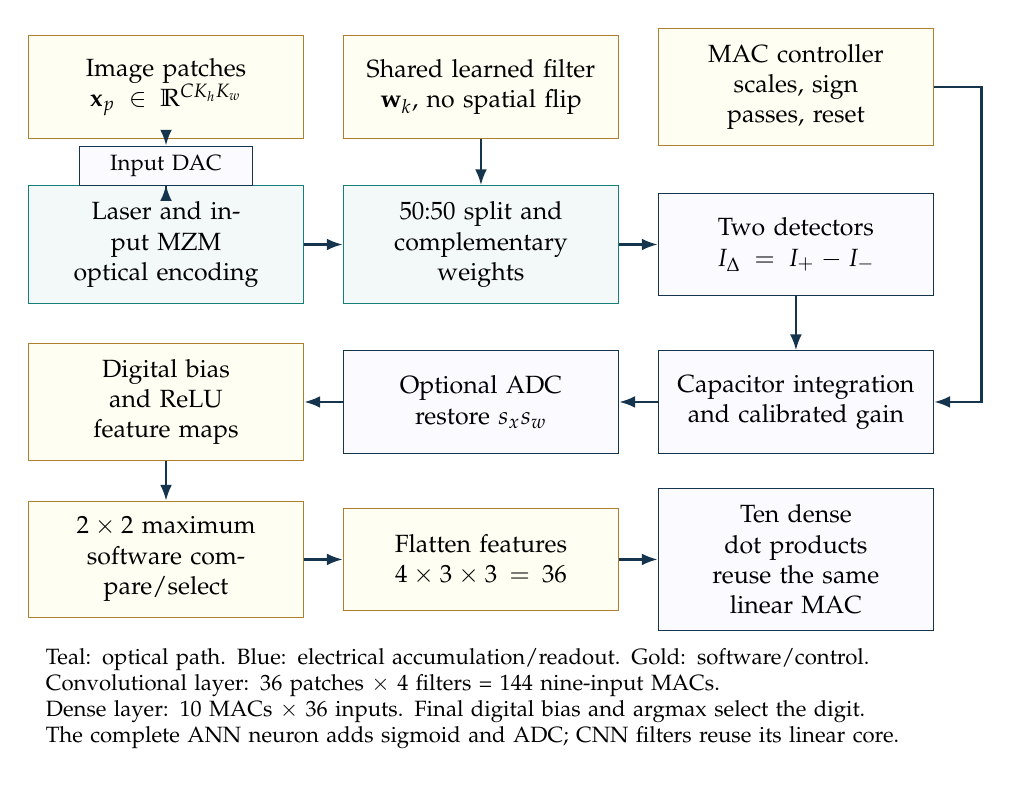
\begin{tikzpicture}[font=\small,
box/.style={draw=navy,align=center,text width=31mm,minimum height=13mm,inner sep=2mm},
sw/.style={box,draw=gold,fill=yellow!5},
op/.style={box,draw=teal,fill=teal!5},
el/.style={box,fill=blue!2},
arr/.style={-{Latex[length=2mm]},thick,draw=navy}]
\node[sw](patch)at(0,0){Image patches\\$\mathbf x_p\in\mathbb R^{C K_hK_w}$};
\node[sw](kernel)at(4,0){Shared learned filter\\$\mathbf w_k$, no spatial flip};
\node[sw](control)at(8,0){MAC controller\\scales, sign passes, reset};
\node[op](encode)at(0,-2){Laser and input MZM\\optical encoding};
\node[op](weight)at(4,-2){50:50 split and\\complementary weights};
\node[el](detect)at(8,-2){Two detectors\\$I_\Delta=I_+-I_-$};
\node[el](integrate)at(8,-4){Capacitor integration\\and calibrated gain};
\node[el](readout)at(4,-4){Optional ADC\\restore $s_xs_w$};
\node[sw](activation)at(0,-4){Digital bias and ReLU\\feature maps};
\node[sw](pool)at(0,-6){$2\times2$ maximum\\software compare/select};
\node[sw](flat)at(4,-6){Flatten features\\$4\times3\times3=36$};
\node[el](dense)at(8,-6){Ten dense dot products\\reuse the same linear MAC};
\node[el,text width=21mm,minimum height=5mm,inner sep=.5mm,font=\footnotesize](dac)at(0,-1){Input DAC};
\draw[arr](patch)--(dac);\draw[arr](dac)--(encode);
\draw[arr](kernel)--(weight);
\draw[arr](control.east)--++(.6,0)|-(integrate.east);
\draw[arr](encode)--(weight);
\draw[arr](weight)--(detect);
\draw[arr](detect)--(integrate);
\draw[arr](integrate)--(readout);
\draw[arr](readout)--(activation);
\draw[arr](activation)--(pool);
\draw[arr](pool)--(flat);
\draw[arr](flat)--(dense);
\node[align=left,text width=111mm,anchor=north west,font=\footnotesize]at(-1.65,-7){
Teal: optical path. Blue: electrical accumulation/readout. Gold: software/control.\\
Convolutional layer: 36 patches $\times$ 4 filters = 144 nine-input MACs.\\
Dense layer: 10 MACs $\times$ 36 inputs. Final digital bias and argmax select the digit.\\
The complete ANN neuron adds sigmoid and ADC; CNN filters reuse its linear core.};
\end{tikzpicture}
\end{document}
